% Agentsensus -- ICLR submission draft.
%
% Numbers are not typed here. % generated by experiments/build_paper_latex.py -- do not edit
\newcommand{\ConsSimNew}{974}
\newcommand{\ConsShPct}{19\%}
\newcommand{\ConsAffPct}{97\%}
\newcommand{\GaSimNew}{1251}
\newcommand{\CoSimNew}{1455}
\newcommand{\ShRange}{14--28\%}
\newcommand{\AffRange}{94--99\%}
\newcommand{\MaxOwners}{10}
\newcommand{\SaveRange}{22--44\%}
\newcommand{\GoalLo}{0.96}
\newcommand{\GoalHi}{0.99}
\newcommand{\QualityLeads}{4}
\newcommand{\QualityCells}{16}
\newcommand{\AblOnEntries}{6,590}
\newcommand{\AblOffEntries}{20,669}
\newcommand{\AblFactor}{3.1}
\newcommand{\AblOffAff}{94\%}
\newcommand{\AblOnAff}{93\%}
\newcommand{\GoallessLo}{0.5\%}
\newcommand{\GoallessHi}{1.6\%}
 defines a macro for every
% quantity the prose quotes, and the three tables are generated files; both
% come from experiments/build_paper_latex.py, so re-run it after a rerun and
% the paper follows the data.
%
% Expects the ICLR style files (iclr2026_conference.sty, .bst, fancyhdr.sty,
% math_commands.tex) that ship with the Overleaf ICLR template.

\documentclass{article}
\usepackage{iclr2026_conference,times}

\usepackage{amsmath,amssymb}
\usepackage{graphicx}
\usepackage{booktabs}
\usepackage{multirow}
\usepackage{subcaption}
\usepackage{xcolor}
\usepackage[utf8]{inputenc}
\usepackage{hyperref}
\usepackage{url}

% generated by experiments/build_paper_latex.py -- do not edit
\newcommand{\ConsSimNew}{974}
\newcommand{\ConsShPct}{19\%}
\newcommand{\ConsAffPct}{97\%}
\newcommand{\GaSimNew}{1251}
\newcommand{\CoSimNew}{1455}
\newcommand{\ShRange}{14--28\%}
\newcommand{\AffRange}{94--99\%}
\newcommand{\MaxOwners}{10}
\newcommand{\SaveRange}{22--44\%}
\newcommand{\GoalLo}{0.96}
\newcommand{\GoalHi}{0.99}
\newcommand{\QualityLeads}{4}
\newcommand{\QualityCells}{16}
\newcommand{\AblOnEntries}{6,590}
\newcommand{\AblOffEntries}{20,669}
\newcommand{\AblFactor}{3.1}
\newcommand{\AblOffAff}{94\%}
\newcommand{\AblOnAff}{93\%}
\newcommand{\GoallessLo}{0.5\%}
\newcommand{\GoallessHi}{1.6\%}


\title{Agentsensus: Consensus-Compressed Shared Memory\\for Multi-Agent Story Worlds}

\author{Anonymous authors\\Paper under double-blind review}

\newcommand{\code}[1]{\texttt{\small #1}}

\begin{document}
\maketitle

\begin{abstract}
Multi-agent story-world simulations give every character a private memory
stream, so one shared event is stored once per witness, its copies drift apart
as agents paraphrase and summarize them, and nothing links a courier's report
to the battle it describes. We present \textbf{Agentsensus}, a story-world
simulation framework whose long-term memory is a single store in which
\emph{sharing is computed rather than assumed}. Each deposit is atomized into
self-contained statements; a statement close to an existing one is put to an
LLM equivalence judge and, if the two are equivalent, merged into one record
whose \emph{owner set} is the union of its witnesses. Statements split from one
deposit are cross-linked, and recall expands one hop along those links.
Ownership stays scoped---an agent recalls only what it owns---so compression
never leaks knowledge between characters, and every mechanism runs inside
\code{remember} and \code{recall}, the only two memory operations agents
demonstrably use: across two models and four backends, discretionary memory
management was invoked zero times. Across four worlds---two classical Chinese
novels, \emph{Hamlet}, and a real-world conflict timeline---run for 40 to 80
rounds against three per-agent memory baselines under an equal-granularity
protocol, consensus writes \SaveRange{} fewer entries than the closest baseline
and is the only backend whose memories become shared (\ShRange{} multi-owner,
single records reaching \MaxOwners{} witnesses) and linked (\AffRange{}), at
judged continuation quality indistinguishable from the baselines. The memory
substrate alone recovers the story's social organization: agents who converse
overlap in memory an order of magnitude more than those who do not.
\end{abstract}

\section{Introduction}

A story-world simulation places dozens of LLM-driven characters in a world with
places, objects and documents, and lets a narrative emerge from what they say
and do to one another \citep{park2023generative,ran2025bookworld}. Unlike a
task-solving multi-agent system, where the team is judged on an answer it
produces \citep{wu2023autogen,hong2024metagpt,qian2024chatdev}, such a world is
judged on what it \emph{accumulates}: who learned what, when, and from whom.
Memory is therefore not a component of these systems but their substrate. It is
also the component that scales worst: a novel-seeded world starts with thousands
of canonical events already deposited, adds several hundred more per hundred
rounds, and must serve retrieval to every character at every round.

The dominant design, established by Generative Agents
\citep{park2023generative} and inherited by most subsequent frameworks
\citep{ran2025bookworld,zhang2024memsurvey}, gives each character a private,
append-only stream scored by recency, importance and relevance. This is faithful
to individual cognition, but as the substrate of a \emph{shared} world it
creates three structural problems, each worsening as the world grows.

\paragraph{P1: witness-multiplied redundancy.} Every shared experience is stored
once per participant: a war council of ten officers produces ten near-identical
records, and a novel-seeded world multiplies this by thousands of canonical
events. Storage, embedding cost and index size scale with the number of
\emph{witnesses} rather than of \emph{events}.

\paragraph{P2: fragmented, divergence-prone world knowledge.} The same event
exists as $N$ independently-worded copies that drift further apart as agents
paraphrase and reflect. No mechanism reconciles them, no record knows its
counterparts exist, and nothing connects a courier's report to the battle it
describes. The connective tissue of the story exists nowhere in the memory
substrate, so retrieval returns one agent's partial view even when the
collective holds the full picture.

\paragraph{P3: memory management that agents never perform.} Stream designs
expose maintenance operations---linking, revising, forgetting---and rely on
agents to use them. Empirically they do not: across two models and all four
backends we test, agents issued \emph{zero} calls to every discretionary
memory-management action, even with documentation, worked examples and an
id-free interface (\S\ref{sec:nomgmt}).

\paragraph{Our approach.} Agentsensus answers all three with one architectural
commitment: \textbf{the world's memory is a single store, and sharing is
computed, not assumed}. Memories stay owner-scoped---an agent recalls only what
it owns, so a shared store is not a shared mind---but when two agents record the
same event, an equivalence mechanism folds the records into one entry owned by
both. This is deduplication with a semantic rather than lexical criterion,
closer to record linkage \citep{fellegi1969record} and semantic corpus
deduplication \citep{abbas2023semdedup} than to caching, and it addresses P1 and
the divergence half of P2. Pieces split from one compound deposit are
automatically cross-linked, and recall expands one hop along those links into
what the caller also owns, giving the store the connective tissue P2 demands
without an agent ever building a graph. Because of P3, \emph{every} mechanism
runs inside \code{remember} and \code{recall} themselves.

\paragraph{Contributions.}
\begin{itemize}
\item A story-world simulation framework with a deterministic round-barrier
  scheduler, passive environments and information carriers, kernel-held
  conversation threads with distance-delayed delivery, and full-system
  checkpoints enabling bit-for-bit resumption.
\item A \textbf{consensus-compressed shared memory}: self-contained atomization,
  semantic-prefilter plus LLM-judged equivalence merging with owner-set union,
  automatic affiliation of split pieces, and auto-expanding owner-scoped recall.
\item An \textbf{equal-granularity, simulation-only evaluation protocol} against
  three faithful baseline reimplementations, applied to four worlds spanning two
  languages, three genres and both human and institutional actors.
\item A three-layer \textbf{case-study methodology} quantifying how the emergent
  memory structure tracks the story's social structure.
\item Two \textbf{negative results} that constrain how such systems should be
  designed and evaluated: agents never perform discretionary memory management,
  so structure must be mechanized; and judged narrative quality is insensitive
  to the memory architecture at this scale.
\end{itemize}

\section{Related Work}

\paragraph{Memory for a single agent.} Generative Agents
\citep{park2023generative} established the stream scored by recency, importance
and relevance and compressed into reflections. Variants change what is stored or
how it is maintained rather than who owns it: MemGPT \citep{packer2023memgpt}
pages context like an operating system, MemoryBank \citep{zhong2024memorybank}
decays it on a forgetting curve, Reflexion \citep{shinn2023reflexion} persists
verbal self-feedback, and A-MEM \citep{xu2025amem} links an agent's notes into an
evolving network. A survey of the area \citep{zhang2024memsurvey} finds the same
shape throughout: the memory belongs to one agent. Agentsensus keeps this
machinery but makes \emph{ownership} a property of a record rather than of a
store, which lets one record belong to several agents at once.

\paragraph{Multi-agent systems and shared state.} AutoGen
\citep{wu2023autogen}, CAMEL \citep{li2023camel}, MetaGPT
\citep{hong2024metagpt} and ChatDev \citep{qian2024chatdev} organize LLMs into
teams whose shared state is the conversation. That is adequate when a team works
a task to completion; a story world runs for hundreds of rounds, and no
transcript survives as a retrieval substrate at that length.

\paragraph{Memory shared across agents.} G-Memory \citep{zhang2025gmemory}
organizes a system's history into an insight/query/interaction hierarchy;
Collaborative Memory \citep{rezazadeh2025collaborative} shares fragments under
dynamic access control. Both are our baselines. Both keep every contributor's
record intact and mediate \emph{access} to them; neither merges records that say
the same thing across contributors. Consensus compression changes the number of
records rather than their visibility, and the owner set it produces is an access
policy that is derived rather than configured.

\paragraph{Deduplication and grounding.} Record linkage
\citep{fellegi1969record} formalized deciding whether two records denote one
entity; semantic deduplication \citep{abbas2023semdedup} showed embedding-space
near-duplicates can be removed without loss. What our setting adds is that the
duplicate carries a \emph{witness}: merging is also a statement that two
characters share a belief, which is why the merged record keeps a set of owners.
The psycholinguistic notion of grounding \citep{clark1991grounding} is the
phenomenon our owner sets approximate mechanically.

\paragraph{Retrieval over graphs.} RAG \citep{lewis2020rag} and its
graph-structured variants---HippoRAG \citep{gutierrez2024hipporag}, GraphRAG
\citep{edge2024graphrag}---build structure over a \emph{static} corpus in an
indexing pass with global knowledge of the documents. Our graph is built
incrementally at deposit time by agents who cannot see the store.

\paragraph{Story worlds and character agents.} Story generation has largely been
a planning problem \citep{mirowski2023dramatron,yang2022re3,yang2023doc};
character agents fit a model to one persona \citep{shao2023characterllm}.
Between them sit simulated worlds \citep{park2023generative,park2024thousand,
hua2023waragent}, and BookWorld \citep{ran2025bookworld}, which builds an agent
society from a novel---the same motivation as our sedimentation stage.
Agentsensus differs in what it puts under test: not the story that comes out,
but the memory substrate it comes from.

\section{The Agentsensus framework}

\begin{figure}[t]
\centering
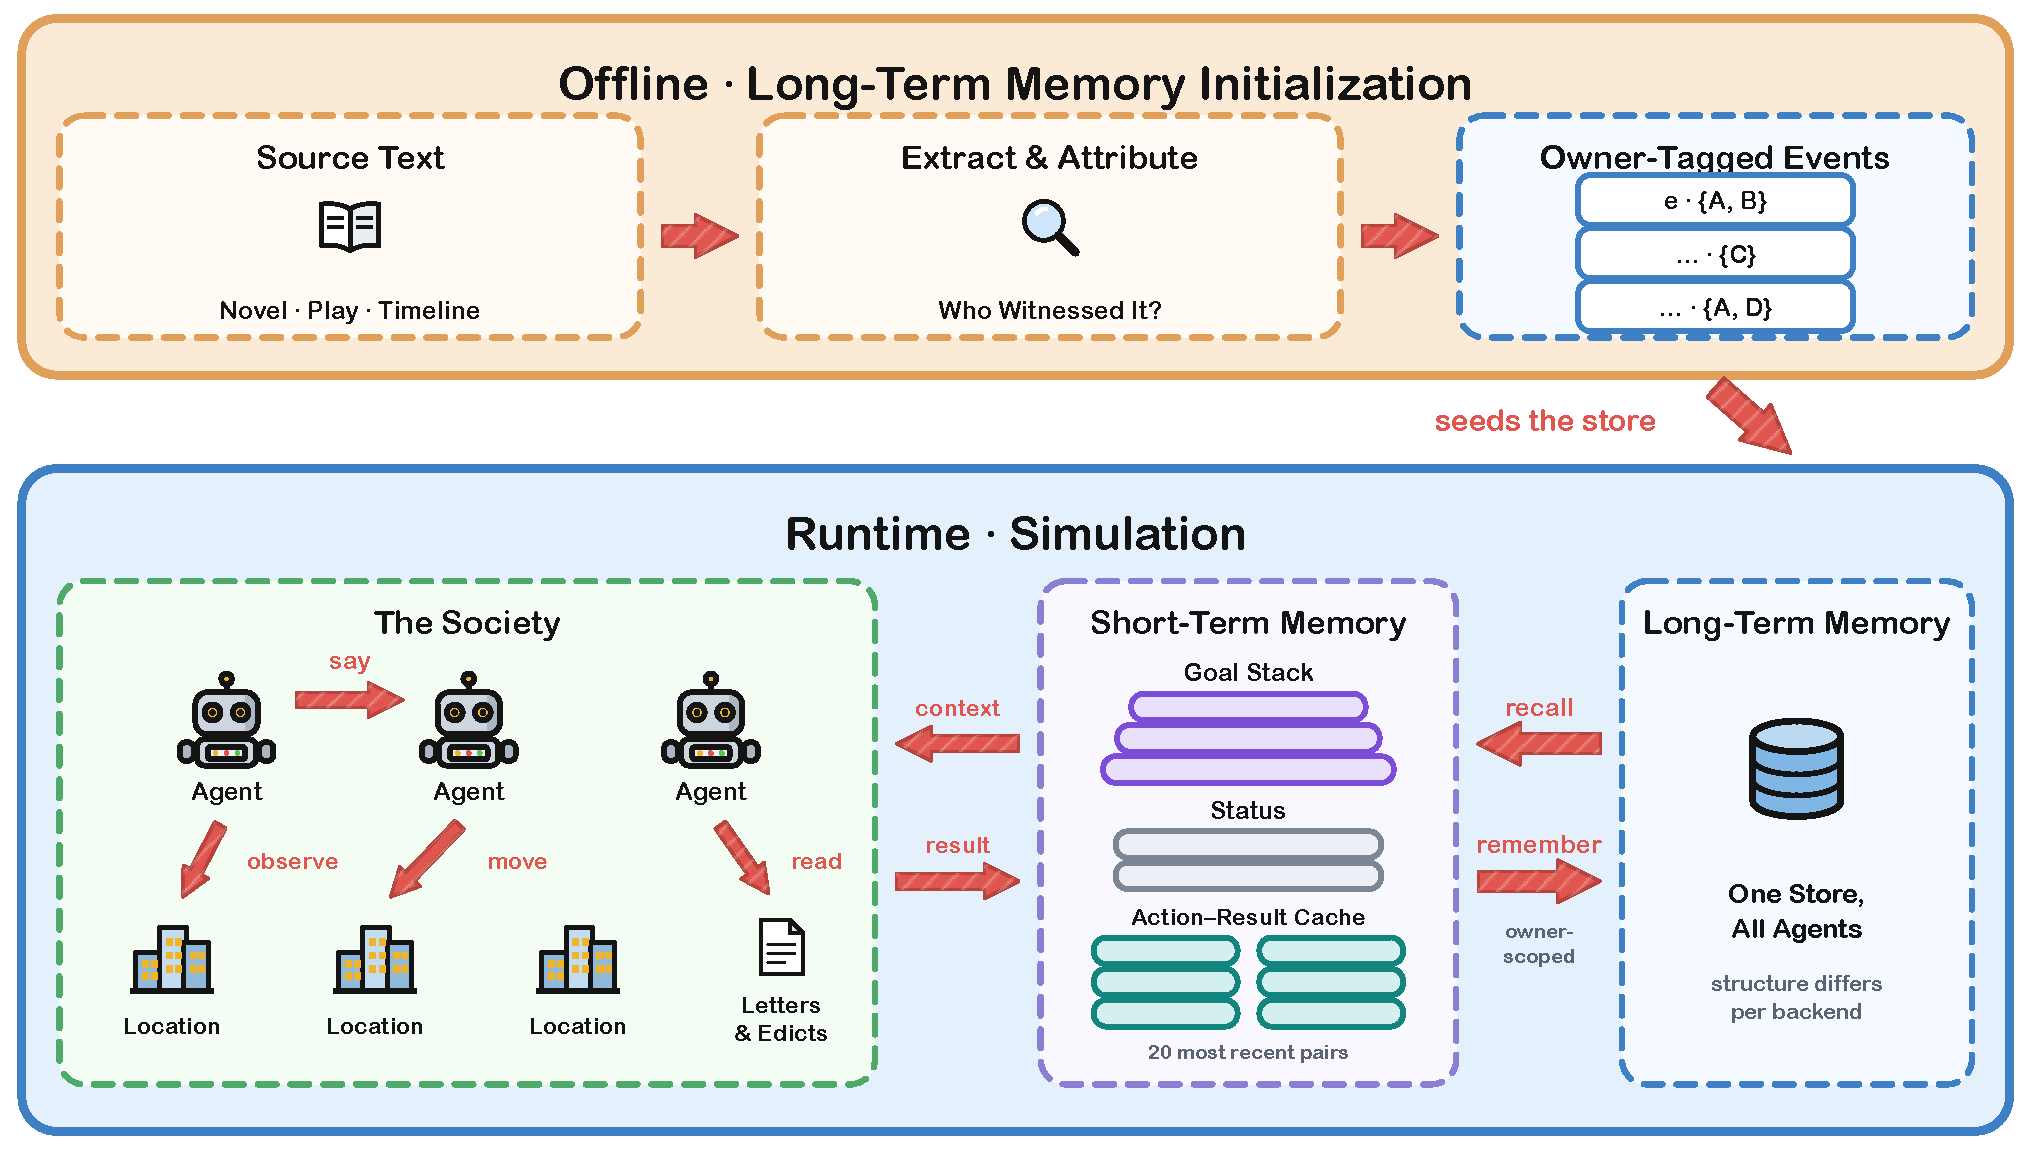
\includegraphics[width=\textwidth]{figures/framework.pdf}
\caption{The framework shared by all four backends. A source text is sedimented
into owner-tagged events that seed one long-term memory store; a round-barrier
kernel then steps every awake agent, and the actions they take deposit into and
retrieve from that store. Only the box marked \emph{memory} differs between the
four systems compared in this paper.}
\label{fig:framework}
\end{figure}

\subsection{World model and round-barrier kernel}
Agents are of three kinds. \emph{Characters} are schedulable and act;
\emph{environments} (places) own memories but never act; \emph{information
carriers} (letters, edicts, scripts) hold text that a character can read. A
round is a barrier: every awake agent observes, decides and acts against the
same world state, and effects become visible in the next round, so a round's
outcome does not depend on the order agents were stepped in. Messages are held
by the kernel as conversation threads, delivered with a delay proportional to
distance, so a letter takes rounds to arrive.

\subsection{Sedimentation}
Before simulation, the source text is turned into a world: a cast, a map,
carriers, and a memory store seeded with what those characters would already
know, each memory tagged with the agents that witnessed it. This is what makes
the redundancy of P1 measurable---the same canonical event arrives with several
owners.

\subsection{The consensus shared memory}
\label{sec:consensus}
A deposit \code{remember(agent, text)} is atomized into self-contained
statements capped at a token budget. Each statement is embedded and matched
against the whole store; candidates above a cosine threshold ($0.70$, top $5$)
go to an LLM judge, which either names an equivalent record or declines. On a
match, the record's owner set becomes the union of the two, its affiliated set
the union, and the shorter of the two texts is kept; on no match, a new record
is written. Statements atomized from one deposit are mutually affiliated, which
is where the memory graph comes from. Recall is owner-scoped and expands one hop
along affiliation into records the caller also owns.

\subsection{How the four designs differ}
\begin{figure}[t]
\centering

\includegraphics[width=\textwidth]{figures/backends.pdf}
\caption{The long-term memory structure of the four backends: private streams
with importance scores and a reflection tree; a two-tier interaction/insight
graph; an access-controlled single store; and the consensus store, whose records
carry an owner set and affiliation edges.}
\label{fig:backends}
\end{figure}
Generative-Agents keeps a private stream per agent with importance scores and a
reflection tree. G-Memory keeps interaction and insight tiers joined by
\code{derived\_from} edges and retrieves at both levels. Collaborative keeps one
store partitioned by an access-control list. Only consensus merges records
across agents.

\section{Experimental setup}
\label{sec:setup}

\paragraph{Worlds.} Three Kingdoms (\emph{sanguo yanyi}) and Dream of the Red
Chamber (\emph{honglou meng}), sedimented from chapters 1--40 and run for 80
rounds; \emph{Hamlet}, sedimented from Acts I--III and run for 40; and a
Russia--Ukraine timeline through 2024-04, run for 40, whose agents are
institutions rather than people. The remainder of each work is held out as the
reference a continuation is scored against.

\paragraph{Baselines.} Faithful reimplementations of Generative-Agents-style
streams, G-Memory and Collaborative Memory, all sharing our kernel, personas,
scenarios and vector store, so the memory mechanism is the only difference.

\paragraph{Equal granularity.} Every backend routes \code{remember} through the
\emph{same} atomizer with the same self-containment requirement, so entry counts
are directly comparable and the only remaining difference is what each mechanism
does with identical atoms. All counts are simulation-only: the seeded history is
excluded, since it is identical by construction.

\paragraph{Metrics.} Structural quantities (entries, multi-owner fraction,
affiliated fraction, merge depth) are deterministic. Continuation quality is
LLM-judged, three scorings each: \emph{grounding}, the fraction of the run's own
events consistent with canon; \emph{trajectory}, agreement of ten principals'
arcs with the held-out span; \emph{narrative}, a 1--5 rubric; and \emph{goal
pursuit}, the fraction of an agent's actions serving a goal it had itself pushed.
The first three read a rendered screenplay of the run---one language, an order of
magnitude smaller than the raw log---and the fourth reads the event log, since
goal management never becomes a dramatizable beat.

\section{Results}

\subsection{Footprint and structure}
\label{sec:structure}

\begin{table}[t]
\centering
\caption{Simulation-written memory at equal granularity. Consensus writes the
fewest entries in every world and is the only backend whose memories acquire
owners or links; the baselines are at exactly zero on both by construction.}
\label{tab:footprint}
% generated
\begin{tabular}{lrrr}
\toprule
Backend & Sediment & Sim & Total \\
\midrule
\multicolumn{4}{l}{\emph{Three Kingdoms --- fiction, 80 rounds, 6,052 source events}} \\
\quad Consensus & \textbf{6,051} & \textbf{974} & 7,025 \\
\quad Gen.\ Agents & 20,896 & 1,251 & 22,147 \\
\quad G-Memory & 27,156 & 1,434 & 28,590 \\
\quad Collaborative & 19,856 & 1,455 & 21,311 \\
\midrule
\multicolumn{4}{l}{\emph{Red Chamber --- fiction, 80 rounds, 6,506 source events}} \\
\quad Consensus & \textbf{6,506} & \textbf{438} & 6,944 \\
\quad Gen.\ Agents & 27,306 & 785 & 28,091 \\
\quad G-Memory & 37,124 & 882 & 38,006 \\
\quad Collaborative & 26,681 & 789 & 27,470 \\
\midrule
\multicolumn{4}{l}{\emph{Russia--Ukraine --- real world, 40 rounds, 1,533 source events}} \\
\quad Consensus & \textbf{1,533} & \textbf{814} & 2,347 \\
\quad Gen.\ Agents & 9,492 & 1,268 & 10,760 \\
\quad G-Memory & 14,346 & 1,191 & 15,537 \\
\quad Collaborative & 8,493 & 1,091 & 9,584 \\
\midrule
\multicolumn{4}{l}{\emph{Hamlet --- fiction, 40 rounds, 1,135 source events}} \\
\quad Consensus & \textbf{1,135} & \textbf{130} & 1,265 \\
\quad Gen.\ Agents & 5,819 & 200 & 6,019 \\
\quad G-Memory & 7,068 & 193 & 7,261 \\
\quad Collaborative & 5,310 & 214 & 5,524 \\
\bottomrule
\end{tabular}

\end{table}

\begin{figure}[t]
\centering
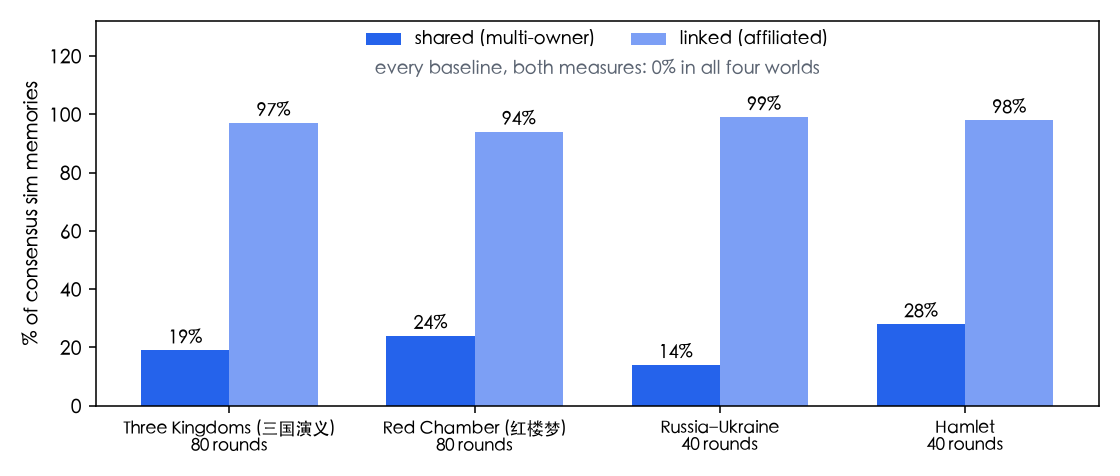
\includegraphics[width=0.85\textwidth]{figures/structure_all.png}
\caption{Sharing and linking across the four worlds. Only consensus is nonzero
on either axis.}
\label{fig:structure}
\end{figure}

At equal granularity consensus writes \SaveRange{} fewer entries than the
closest baseline in each world (Table~\ref{tab:footprint}), because merging
folds witnesses together rather than storing them separately. It is also the
only backend whose memories become shared (\ShRange{} multi-owner) or linked
(\AffRange{}); the baselines sit at zero on both, by construction rather than by
tuning. The deepest merge reaches \MaxOwners{} witnesses---a presidential
air-defense directive co-owned by the president, his chief of staff and adviser,
the interior minister, the air-force and intelligence commanders, and the
security service.

\subsection{Structure compounds with horizon}
Sharing is not a fixed property but a function of how long the world has run:
Red Chamber, run at four horizons, goes 13\%$\to$20\%$\to$23\%$\to$24\% at
rounds 10/40/60/80, and Russia--Ukraine 6\%$\to$9\%$\to$14\% at 10/20/40. Later
deposits meet a store that already holds their equivalents, so the compression
compounds rather than saturating early.

\subsection{Continuation quality}
\label{sec:quality}

\begin{table}[t]
\centering
\caption{Continuation quality, means over three scorings. No backend leads
everywhere and no world has one leader on all four metrics.}
\label{tab:quality}
\resizebox{\textwidth}{!}{% generated
\begin{tabular}{llrrrr}
\toprule
World & Backend & Grounding & Trajectory & Narrative & Goal \\
\midrule
\multirow{4}{*}{Three Kingdoms} & Consensus & 0.88\tiny$\pm$0.02 & 0.87\tiny$\pm$0.02 & 4.08\tiny$\pm$0.12 & 0.98\tiny$\pm$0.00 \\
 & Gen.\ Agents & 0.93\tiny$\pm$0.01 & 0.82\tiny$\pm$0.02 & 4.00\tiny$\pm$0.00 & 0.99\tiny$\pm$0.00 \\
 & G-Memory & 0.88\tiny$\pm$0.01 & 0.87\tiny$\pm$0.01 & 3.83\tiny$\pm$0.12 & 0.99\tiny$\pm$0.00 \\
 & Collaborative & 0.89\tiny$\pm$0.02 & 0.89\tiny$\pm$0.01 & 3.92\tiny$\pm$0.12 & 0.97\tiny$\pm$0.01 \\
\midrule
\multirow{4}{*}{Red Chamber} & Consensus & 0.92\tiny$\pm$0.02 & 0.86\tiny$\pm$0.02 & 4.00\tiny$\pm$0.00 & 0.98\tiny$\pm$0.01 \\
 & Gen.\ Agents & 0.88\tiny$\pm$0.04 & 0.87\tiny$\pm$0.02 & 4.25\tiny$\pm$0.00 & 0.98\tiny$\pm$0.01 \\
 & G-Memory & 0.93\tiny$\pm$0.01 & 0.89\tiny$\pm$0.03 & 4.00\tiny$\pm$0.00 & 0.99\tiny$\pm$0.01 \\
 & Collaborative & 0.95\tiny$\pm$0.03 & 0.92\tiny$\pm$0.01 & 4.25\tiny$\pm$0.00 & 0.98\tiny$\pm$0.01 \\
\midrule
\multirow{4}{*}{Russia--Ukraine} & Consensus & 0.94\tiny$\pm$0.01 & 0.85\tiny$\pm$0.03 & 3.83\tiny$\pm$0.12 & 0.99\tiny$\pm$0.00 \\
 & Gen.\ Agents & 0.97\tiny$\pm$0.01 & 0.77\tiny$\pm$0.01 & 4.00\tiny$\pm$0.00 & 0.97\tiny$\pm$0.01 \\
 & G-Memory & 0.94\tiny$\pm$0.03 & 0.82\tiny$\pm$0.02 & 4.00\tiny$\pm$0.00 & 0.97\tiny$\pm$0.01 \\
 & Collaborative & 0.97\tiny$\pm$0.01 & 0.81\tiny$\pm$0.03 & 4.25\tiny$\pm$0.20 & 0.97\tiny$\pm$0.00 \\
\midrule
\multirow{4}{*}{Hamlet} & Consensus & 0.84\tiny$\pm$0.06 & 0.65\tiny$\pm$0.02 & 3.50\tiny$\pm$0.20 & 0.96\tiny$\pm$0.02 \\
 & Gen.\ Agents & 0.84\tiny$\pm$0.04 & 0.64\tiny$\pm$0.02 & 3.25\tiny$\pm$0.20 & 0.99\tiny$\pm$0.00 \\
 & G-Memory & 0.89\tiny$\pm$0.03 & 0.53\tiny$\pm$0.03 & 3.67\tiny$\pm$0.24 & 0.98\tiny$\pm$0.01 \\
 & Collaborative & 0.83\tiny$\pm$0.02 & 0.51\tiny$\pm$0.04 & 3.33\tiny$\pm$0.12 & 0.98\tiny$\pm$0.01 \\
\bottomrule
\end{tabular}
}
\end{table}

Of the \QualityCells{} world-metric cells, consensus is best in \QualityLeads{}
and trails elsewhere by margins the size of the spread across three scorings of
the same text. We report this as a wash rather than a win: compression neither
buys judged quality nor costs it, and the case for consensus rests on
\S\ref{sec:structure}. Goal pursuit saturates at \GoalLo{}--\GoalHi{} for every
backend---the goal stack is in every prompt and only \GoallessLo{}--\GoallessHi{}
of actions are taken with no goal held---so it certifies the agent loop and
separates nothing.

\subsection{The memory graph tracks the social graph}
Three layers of the same run can be compared: who talked to whom, which memories
are affiliated, and who owns what. Agents who converse overlap in memory an
order of magnitude more than those who do not, linked memories share witnesses
far more often than unlinked ones, and cross-agent memory links run almost
exclusively between conversing pairs. The structure the mechanism produces is
therefore not incidental: the story's social organization can be read off the
memory substrate alone.

\subsection{Agents do not manage memory}
\label{sec:nomgmt}
Across all four backends and both models tested, agents issued zero calls to
every discretionary memory-management action---linking, forgetting, revising,
graph traversal by id---while calling \code{remember} and \code{recall}
constantly. This is why every structural mechanism in \S\ref{sec:consensus} runs
inside those two operations. A memory architecture that depends on agent-side
curation does not acquire structure in practice, however well the operations are
designed.

\subsection{Ablation}
\label{sec:ablation}

\begin{table}[t]
\centering
\caption{One factor at a time from the published configuration, consensus on
Three Kingdoms, 40 rounds. All four quality metrics here read the event log, so
they compare across cells rather than against Table~\ref{tab:quality}.}
\label{tab:ablation}
\resizebox{\textwidth}{!}{% generated
\begin{tabular}{llrrrrrrrr}
\toprule
Merge & Cache & Store & Sim & Shared & Linked & Grnd & Traj & Narr & Goal \\
\midrule
on & fifo \emph{(published)} & 6,590 & 539 & 19\% & 93\% & 0.92 & 0.89 & 4.17 & 0.97 \\
on & relevance & 6,674 & 623 & 21\% & 96\% & 0.93 & 0.83 & 4.33 & 0.99 \\
on & hybrid & 6,670 & 619 & 18\% & 96\% & 0.94 & 0.90 & 4.25 & 0.98 \\
\textbf{off} & fifo & 20,669 & 813 & 0\% & 94\% & 0.92 & 0.82 & 4.00 & 0.96 \\
\bottomrule
\end{tabular}
}
\end{table}

\begin{figure}[t]
\centering
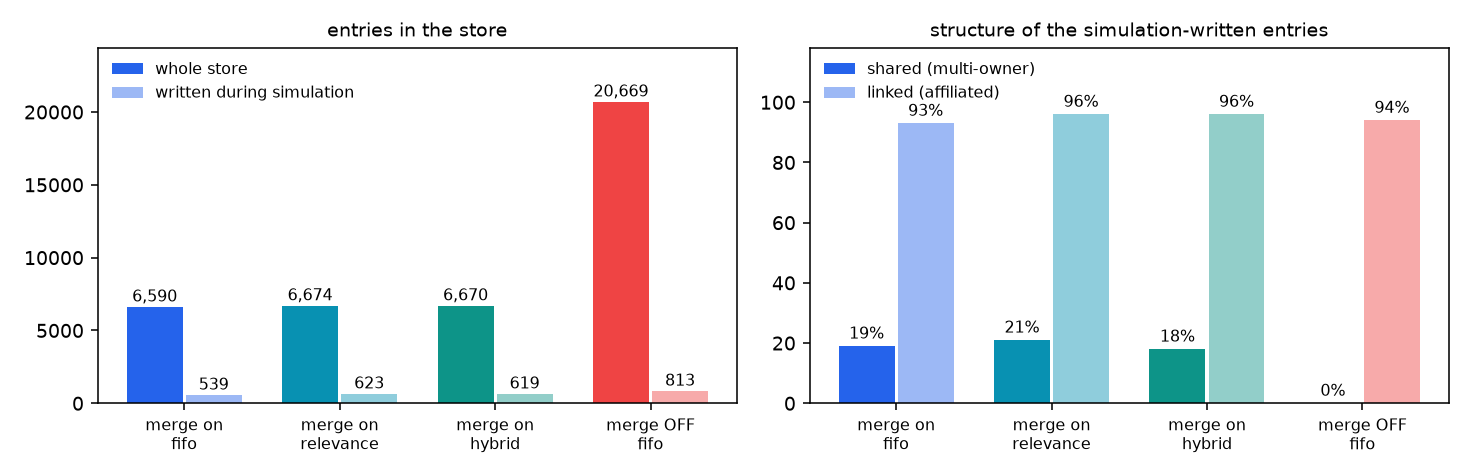
\includegraphics[width=\textwidth]{figures/ablation.png}
\caption{What each knob does. Left: entries in the whole store and in the
simulation-written part. Right: the two structural properties. Turning the merge
off is the only change visible in either panel.}
\label{fig:ablation}
\end{figure}

Disabling the merge multiplies the store by \AblFactor{}$\times$
(\AblOffEntries{} entries against \AblOnEntries{}) and takes sharing to exactly
zero: P1 measured against its own control rather than against a different
system. Two findings correct the paper's own framing. First, sharing and linking
are \emph{separable}: with the merge off, linking is still \AblOffAff{}, against
\AblOnAff{} published, because links come from the atomizer rather than from the
merge. Second, the short-term cache policy is not a research variable---
relevance and hybrid eviction leave every structural quantity where FIFO leaves
it, at 15--19\% more wall-clock. The quality columns do not separate on the merge
either.

\section{Discussion and limitations}
Consensus compression buys structure and footprint at no measurable cost in
judged behaviour. The mechanism has three costs we can name. Merging keeps the
shorter of two equivalent texts, discarding detail the longer one carried, and we
have not isolated what that costs. Auto-expansion is uncapped, enriching context
but growing prompts. And equivalence is decided by a single LLM call over five
candidates with no verification, so a wrong merge is permanent; the judge sees
text alone, without owners or time, which makes routine repeated events the
plausible failure mode. Every number here comes from single stochastic runs; the
one cell we reran replicated to within 1\%.

\section{Conclusion}
Agentsensus treats a story world's memory as a single consensus store: equivalent
memories merge across witnesses, split memories link into a graph, and recall
walks that graph automatically. Across four worlds this yields the smallest
memory footprint at equal granularity, the only shared and linked memory
structure among four backends, and an emergent graph that mirrors the story's
social structure, while judged continuation quality stays within noise of the
baselines. The broader lesson is that memory structure in multi-agent systems
must be mechanized, not delegated: agents reliably use only \code{remember} and
\code{recall}, so that is where the structure has to live.

\bibliography{references}
\bibliographystyle{iclr2026_conference}

\appendix
\section{Appendix}

\subsection{How the scenes were cut}
\begin{figure}[h]
\centering
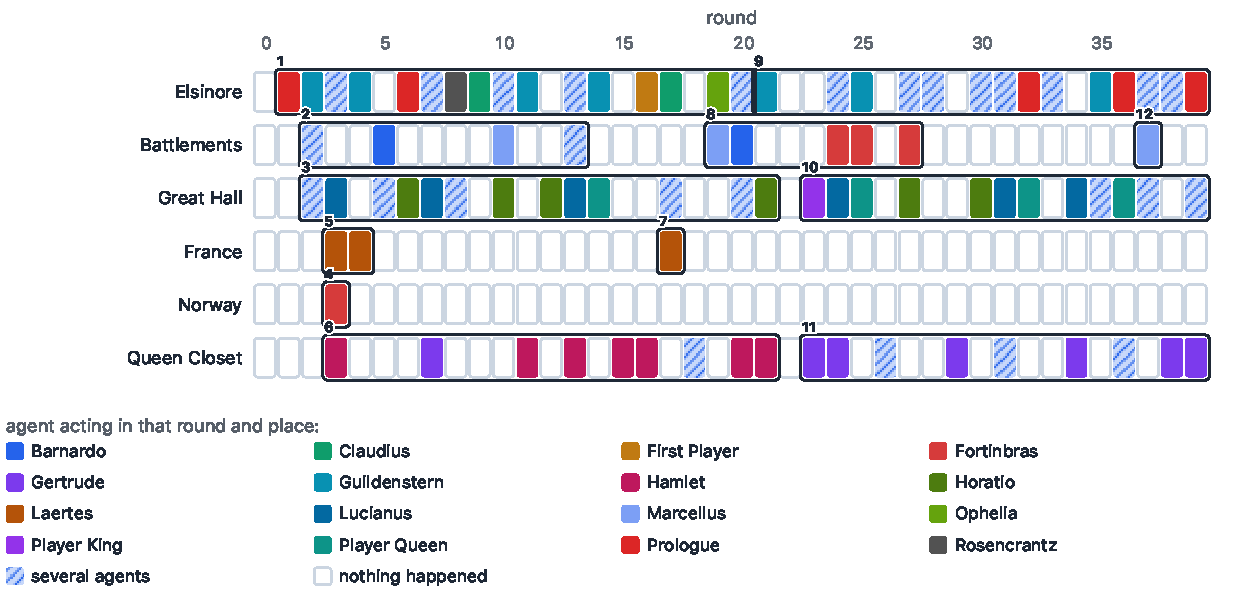
\includegraphics[width=\textwidth]{figures/grid_hamlet.pdf}
\caption{Every cell is one round at one place, coloured when an agent acted
there and white when nothing did; hatched cells are rounds where several agents
acted in the same place. Outlined rectangles are the scenes the screenplay
renderer produced.}
\label{fig:grid}
\end{figure}

Further material---the full screenplays of all four worlds, the action census
per backend, per-world scene grids, the language composition of the runs, and
merge-depth distributions---is available in the extended version.

\end{document}
